\section{Modelling the shear correlation functions}
\label{sec:xipm}
A convenient way to infer cosmological information from observational data are the shear correlation functions $\xi_\pm$, which are defined as \[
\xi_\pm = \la \gamma_{\rm t}\gamma_{\rm t}\ra \pm \la \gamma_\times\gamma_\times\ra \, .
\]
They are the prime estimators to quantify a cosmic-shear signal since it is simple to include a weighting of the shear-measurements into the correlation functions and, contrary to the power spectrum, one does not have to worry about the shape of the survey footprint, or masked regions. Cosmologically, given two comoving distance probability distributions of sources $p_i(\chi),p_j(\chi)$, one can compute the shear correlation function from the underlyting matter power spectrum $P_\delta$ via \todo{Citation!}\begin{align}
\label{eq:xipm-pkappa}
\xi_\pm^{ij}(\theta) =& \int_0^\infty \frac{{\rm d}\ell\,\ell}{2\pi}J_{0,4}(\ell\theta)P^{ij}(\ell)\, , \\
\label{eq:pkappa-pdelta/lenseff}
P^{ij}(\ell) =& \frac{9 H_0^4\Omega_{\rm m}^2}{4c^4}\int_0^{\chi_h} {\rm d}\chi\frac{g^i(\chi)g^j(\chi)}{a^2(\chi)}P_\delta\left(\frac{\ell}{f_K(\chi)},\chi\right)\, , \\
\label{eq:lenseff}
g^i(\chi) =& \int_\chi^{\chi_H} {\rm d}\chi'\, p_i(\chi') \frac{f_K(\chi'-\chi)}{f_K(\chi')}\, .
\end{align}
Here, $J_{0,4}$ denote the 0-th and 4-th order Bessel Functions.
\subsection{Using an analytic Model}
\label{sec:xipm_analytic}
For a first simple analysis we will assume that a deeper redshift distribution just yields a stronger shear signal, in the sense that the shear field for a deeper redshift distribution gets multiplied by a weight $W$. While this is not true for a 3-dimensional matter distribution, it should be valid for small variations in redshift. Additionally, we assume that a higher depth does not only lead to a stronger average shear, but also to a higher galaxy number density, implying a correlation between those two quantities.

Let $N^i(\b \theta),N^j(\b\theta)$ be the average weighted number of galaxies per pointing in redshift bins $i$ and $j$ and let $W^i(\b \theta),W^j(\b\theta)$ be the weighting of average shear. The observed correlation function $\xi^{ij,\text{obs}}_\pm(\theta)$ now changes from one of constant depth $\xi_\pm^{ij,\rm{const}}(\theta)$ via (compare Eq. \todo{Take eq. from Hildebrandt et al. (2017)?})
\begin{align}
\xi^{ij,\text{obs}}_\pm(\theta) = & \frac{\la N^i(\bth)N^j(\bthp)\gamma^{i,\rm{obs}}_{\rm t}(\bth)\gamma^{j,\rm{obs}}_{\rm t}(\bthp)\ra }{\la N^i(\bth)N^j(\bthp)\ra} \pm \frac{\la N^i(\bth)N^j(\bthp)\gamma^{i,\rm{obs}}_\times(\bth)\gamma^{j,\rm{obs}}_\times(\bthp)\ra }{\la N^i(\bth)N^j(\bthp)\ra} \nonumber\\
 = & \frac{\la N^i(\bth)N^j(\bthp)W^i(\bth)W^j(\bthp)\ra}{\la N^i(\bth)N^j(\bthp)\ra} \xi_{\pm}^{ij,\rm{const}}(\theta) \, ,
 \label{eq:xipmblub1}
 \end{align}
 where the average $\la\ldots\ra$ represents both an ensemble average as well as an average over the position $\bth$.
 Assuming that depth and galaxy number density of neighbouring pointings are uncorrelated, the only important property of a galaxy pair is whether or not they lie in the same pointing. We want to denote the probability, that a random galaxy pair of separation $\theta$ lies in the same pointing with $E(\theta)$. This function is depicted in Figure \ref{fig:eoftheta_lin}; an exact equation and derivation are given in \ref{sec:model_e}.
 
\begin{figure}
 \centering
 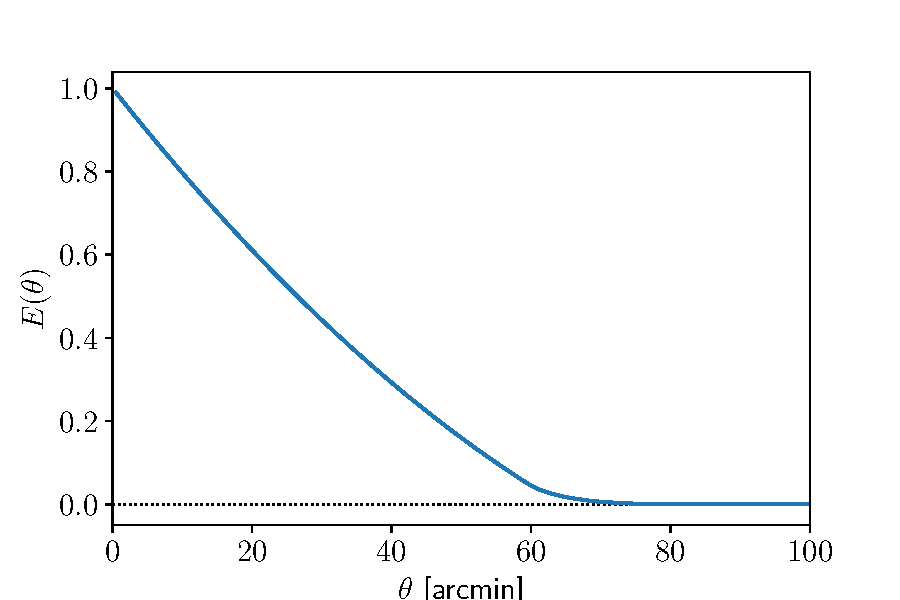
\includegraphics[width=0.5\textwidth]{images/eoftheta.pdf}
 \caption{Probability that a random pair of galaxies of distance $\theta$ lie in the same pointing.}
 \label{fig:eoftheta_lin}
\end{figure}

To compute the modified shear correlation functions, we parametrize the number densities \linebreak$N^{i}(\b \theta)=\la N^{i} \ra [1+n^{i}(\b \theta)]$ and the weight $W^{i}(\b \theta)=1+w^{i}(\b \theta)$ and, as in \eqref{eq:defweightf}, interpret $n^{i}(\b \theta)$ as a function with average $\la n^{i} \ra = 0$, that is constant on each pointing. Without loss of generality we set $\la N^i\ra = 1$. We can see that $\la n^i(\bth)n^j(\bthp)\ra = E(\theta)\la n^i(\bth)n^j(\bth)\ra \equiv E(\theta)\la n^i n^j \ra$ holds and compute:
\begin{align}
&\la N^i(\bth)N^j(\bthp)W^i(\bth)W^j(\bthp)\ra \nonumber\\
&\qquad =  1 + \la n^iw^i\ra + \la n^j w^j\ra + E(\theta)\left[ \la n^in^j\ra + \la n^i w^j \ra  + \la n^jw^i\ra + \la w^iw^j\ra + \la n^in^jw^i\ra + \la n^in^jw^j\ra + \la n^iw^iw^j\ra \right. \nonumber\\
&\qquad\quad \left. + \la n^jw^iw^j\ra + \la n^in^jw^iw^j\ra  \right] 
 \end{align}
Ignoring correlations higher than second order\footnote{It is not inherently obvious that this is a valid assumption. However, after performing both calculations we noticed no difference between the outcomes of both equations.}, and performing the same calculation for the denominator of Eq.\,\eqref{eq:xipmblub1}, we get
 \begin{align}
 \xi^{ij,\rm{obs}}_\pm(\theta) = \frac{1 + \la n^iw^i\ra + \la n^jw^j\ra + E(\theta)\left[\la n^in^j\ra + \la n^iw^j\ra + \la n^j w^i\ra + \la w^iw^j\ra\right]}{1+E(\theta)\la n^i n^j\ra }\xi^{ij,\rm{const}}_\pm (\theta) \, .
 \end{align}
For the calculation of the reference correlation functions $\xi_\pm^{ij}(\theta)$ we distribute the \textit{same} galaxies into our survey, only this time we will not order their weightings $W$ or their number densities $N$ by pointing. We can imagine this by cutting the footprint into infinitesimal elements $\d^2\b\theta$, and redistributing those at random. When we calculate the correlation function of this survey, we note that $\la n^i(\bth)\ra \la n^j(\bthp)\ra = 0$ holds for $\b\theta\neq \b 0$, as the two corresponding infinitesimal elements have uncorrelated weighting and number density. Performing the same calculations as above, this yields a relation between the correlation function of constant optical depth $\xi_\pm^{ij,\rm{const}}$ and the modelled one $\xi_\pm^{ij}$:
\begin{equation}
\xi_\pm^{ij}(\theta) = \left(1+\la n^iw^i\ra + \la n^jw^j\ra \right)\xi_\pm^{ij,\rm{const}}(\theta)\, .
\end{equation}
The ratio of modelled and observed correlation function thus becomes: \begin{equation}
\frac{\xi^{ij}_\pm(\theta)}{\xi_\pm^{ij,\rm{obs}}(\theta)} \approx \frac{1+\la n^iw^i\ra+\la n^jw^j\ra + E(\theta)\la n^in^j\ra}{1 + \la n^iw^i\ra + \la n^jw^j\ra + E(\theta)\left[\la n^in^j\ra + \la n^iw^j\ra + \la n^j w^i\ra + \la w^iw^j\ra\right]}
\, .
\end{equation}
It is interesting to note that $\xi^{ij}_\pm = \xi_\pm^{ij,\rm{obs}}$ holds wherever $E(\theta)=0$, meaning that the correlation function is not affected for large angular scales. Given a set of average redshifts, following \citet{2006APh....26...91V}, we can estimate 
\[
\la |\gamma| \ra \propto \la z \ra ^{0.85}\, .
\]
We shall later see that this approximation is valid for higher tomographic redshift bins $z\gtrsim 0.5$, but starts to break down at lower redshifts. We thus want to construct a model that is valid for an arbitrary distribution of redshifts and does not rely on the assumption of a single lens plane. 
\subsection{Using a semi-analytic Model}
The analysis of data from the Kilo-Degree Survey showed that the redshift-distribution of sources was highly correlated with the depth in the $r$-band. We thus chose to separate the survey into 10 percentiles, sorted by $r$-band depth, meaning that if a pointing had a worse depth than 90\% of the other pointings, it would belong to the first percentile, and so on. For each percentile $m$ and each tomographic redshift bin $i$ we can extract a weighted number of galaxies $N^i_m$ and, in case the pointing overlaps with a spectroscopic survey, a source redshift distribution $p^i_m(z)$. Using \eqref{eq:xipm-pkappa}, we can compute the shear correlation functions $\xi_{\pm,mn}^{ij}(\theta)$ for each set of percentiles $m,n$ and redshift bins $i,j$\footnote{For the calculation of the shear correlation functions we use the \textsc{Nicaea}-program. Among other things, it calculates the shear correlation functions for a given cosmology and source redshift distribution. To estimate the power spectrum on nonlinear scales we use the methods developed by \citet{2012ApJ...761..152T}.}. When we compute the measured shear correlation functions of a survey, we take the weighted average of tangential and cross shears of all pairs of galaxies (\citet{2017MNRAS.465.1454H} give a good overview for the process\todo{Cite the same eq. as above from Hildebrandt et al. (2017)}). If, for a single pair of galaxies, one galaxy lies in the $m$-th percentile of redshift bin $i$ and the second one lies in the $n$-th percentile of redshift bin $j$, then their contribution to the observed correlation functions is, on average, $\xi_{\pm,mn}^{ij}(\theta)$. This means that if we know each of those single correlation functions, we can reconstruct the total correlation functions via a weighted average of the single functions. Formally, we define \[
\xi_\pm^{ij,\rm{obs}}(\theta) = \frac{\sum_{m,n} P_{mn}^{ij}(\theta)\,\xi_{\pm,mn}^{ij}(\theta)}{\sum_{m,n} P_{mn}^{ij}(\theta)}\, ,
\label{eq:def_xiobs}
\]
where $P_{mn}^{ij}$ is the new weighting of the correlation functions. This weighting has to be proportional to the probability that a galaxy pair of distance $\theta$ is of percentiles $m$ and $n$, as well as to the original weighting of these galaxies.\todo{We could completely scratch this derivation and just point to the Appendix; I personally feel that this approach is more intuitive than the more mathematical one of the appendix, but if the paper gets too long we definitely do not need two methods to derive the same equation.}

In this analysis, we will assume an infinitely large survey footprint with an uncorrelated distribution of depth. We will later discuss the validity of these assumptions as well as possible mitigation strategies. For $m\neq n$ we know that the pair of galaxies has to lie in different pointings, which is accounted for by including the factor $[1-E(\theta)]$. Furthermore, the first galaxy has to lie in percentile $m$, the probability of which is $1/10$. The pointing of the second galaxy has to be of percentile $n$; the probability of that is also equal to $1/10$. The impact of such a galaxy pair on the correlation functions scales with the product of the weighted number of galaxies $N_m^i,N_n^j$. We get for $n\neq m$: \[
P_{mn}^{ij}(\theta) = [1-E(\theta)]\frac{1}{100} N_m^i N_n^j\, .
\label{eq:pmnij_corr1}
\]
For the calculation of $P_{mm}^{ij}(\theta)$ we have to account for a different possibility: In case that the galaxy lies in the same pointing [accounted for by the factor $E(\theta)$], it automatically is of the same percentile. We therefore set \[
P_{mm}^{ij}(\theta) = E(\theta)\frac{1}{10} N_m^iN_m^j + [1-E(\theta)]\frac{1}{100} N_m^i N_m^j \, .
\label{eq:pmnij_corr2}
\]
We can then write $P_{mn}^{ij}(\theta)$ as: \[
P_{mn}^{ij}(\theta) = E(\theta)\frac{1}{10} N_m^iN_n^j\,\delta_{mn} + [1-E(\theta)]\frac{1}{100} N_m^i N_n^j \, ,
\label{eq:pmnij_uncorr}
\]
where $\delta_{mn}$ denotes the Kronecker delta.
Inserting this into Eq.\,\eqref{eq:def_xiobs}, we compute
\begin{align}
\xi_{\pm,mn}^{ij,\rm{obs}}(\theta) = & \frac{1}{C}\sum_{m=1}^{10} N_m^i \left\{ E(\theta) N_m^j \xi_{\pm,mm}^{ij}(\theta) + \frac{\big[1-E(\theta)\big]}{10}\sum_{n=1}^{10}N_n^j \xi_{\pm,mn}^{ij}(\theta)\right\}\, ,
\label{eq:correctionfunction1}
\end{align}
with the normalization
\[
C = \sum_{m=1}^{10} N_m^i \bigg[ E(\theta)  N_m^j + \frac{\big[1-E(\theta)\big]}{10}\sum_{n=1}^{10} N_n^j\bigg]\, .
\]
A more mathematically rigorous derivation of this function can be found in Appendix \ref{sec:calc of xipm}.

If we want to compute this for all 5 redshift bins of the KV450-survey, this forces us to calculate 1275 correlation functions and add them, thus yielding potential numerical errors (apart from being computationally expensive). However, if we examine Eq.\,\eqref{eq:lenseff}, we see that the comoving distance distribution of sources factors in linearly. This in turn implies that in Equations \eqref{eq:pkappa-pdelta/lenseff} and \eqref{eq:xipm-pkappa} both source distance distributions factor in linearly. This basically means that, instead of adding correlation functions, we can add their respective redshift distributions and compute the correlation functions of that. In particular, we can define the \textit{combined number of galaxies} $N^i$ and \textit{average redshift distribution} $p^i(z)$ of tomographic bin $i$ as \[
N^i\equiv\sum_m N_m^i\, , \qquad p^i(z) = \frac{\sum_m N_m^i p_m^i(z)}{\sum_m N_m^i} \, .
\]
If we define $\xi^{ij}_\pm$ as the correlation functions between the average redshift distributions $p^i(z)$ and $p^j(z)$, then we observe: \[
\sum_{m,n}N_m^iN_n^j\xi^{ij}_{\pm,mn} = N^iN^j\xi^{ij}_\pm\, .
\]
Consequently, we can apply this to \eqref{eq:correctionfunction1}, yielding
\begin{equation}
\xi_{\pm}^{ij,\rm{obs}}(\theta) = \frac{1}{C}\left\{ E(\theta)\left[\sum_{m=1}^{10} N_m^iN_m^j \xi_{\pm,mm}^{ij}(\theta)\right] +\frac{\big[1-E(\theta)\big]}{10}\xi_\pm^{ij}(\theta)N^iN^j\right\}\, .
\label{eq:correctionfunction2}
\end{equation}
For each set of redshift bins we thus only have to compute eleven correlation functions, which reduces the number of functions to compute from 1275 to 165.
